\documentclass[Main]{subfiles}
\begin{document}


\chapter{Hardware}


\section{Drone}
Dronen vi valgte havde disse prioriteter:
\begin{itemize}
\item Skulle være open source.
\item Skulle have en ordentlig løfteevne.
\item Skulle have udskiftelige dele, såsom propeller, arme, skjold og hardwaresensorer.
\end{itemize}

Der blev set på 3 forskellige droner:
\subsection{Bitcraze}
Det svenske firma Bitcraze har lavet dronen CrazyFlie\cite{BitCraze}, en lille quadrocopter på 19 gram, der kan styres vha. computeren eller en fjernbetjening.
Dronen har mange fine perspektiver, men da den ikke er mere 9 cm fra motor til motor, har den også en meget begrænset løfteevne, og muligheden for at udbygge den er meget lille.

\subsection{Arducopter}
Det amerikanske firma 3D Robotics har lavet dronen 3DR RTF Quad\cite{ArduCopter}, en væsentlig større drone, med 10" propeller, 20 Amp ESC'er (motor kontrol) og 850 $K_v$\cite{Kv} motorer.
Den medfølgende software er skrevet i Arduino (mere om det i afsnit \ref{sec:software}). 
Prisen ligger på 599 USD uden ekstra udstyr.

\subsection{AeroQuad}
Det amerikanske firma AeroQuad har lavet dronen Cyclone\cite{AQ-store}, en næste tilsvarende drone til Arducopters drone, med 12" propeller, 30 Amp ESC'er og 950 $K_v$\cite{Kv} motorer.
Softwaren er ligeledes skrevet i Arudino, og koster kun 550USD.
\\
\\
Da prisen for et bachelorprojekt skal holdes lavest muligt og vi ønskede mest kraft for pengene, blev valget AeroQuads Cyclone model, da denne er 50 USD billigere end Arducopteren og, i modsætning til Bitcraze, kan udbygges med flere sensorer, hvilket gør fremtidige studerende kan udvikle på den.


\section{Valg af trådløs kommunikation}

Der er flere krav til den trådløse sender;

\begin{itemize}
\item Regler
\item Frekvens
\item Data bus
\item Hastighed
\end{itemize}

\subsection{Regler og valg af frekvens}
Der er mange regler inden for trådløs kommunikation, så hvilke frekvenser er lovlige at udnytte uden licens?

Det er de fleste i ISM-båndet, da de er lavet til  Industriel, videnskabelig og medicinsk bånd\fxnote{Torben skrev "Scientific medical" her}. 
Grunden til det ikke er alle er at der er lokale krav, alt efter hvor man er i verden. 
F.eks. har USA meget komplekse krav til 433 MHz\cite[s. 32]{Lov1}.
De meste gængse frekvenser der er kan benyttes i industrien og til hobbybrug er derfor:

\begin{itemize}
\item 433 MHz
\item 868 MHz
\item 915 MHz
\item 2.4 GHz
\item 5.8 GHz
\end{itemize}

Så der skal vælges en frekvens af disse.
Den frekvens der egner sig bedst dette projekt, er den frekvens der rækker længst. 

\begin{figure}[H]
\centering
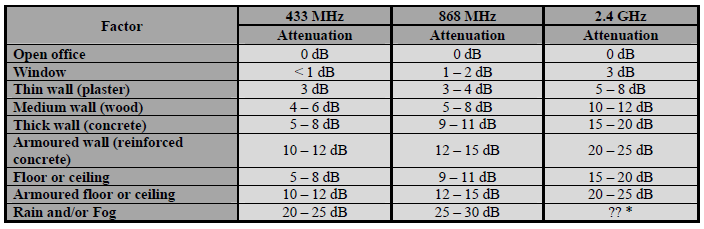
\includegraphics[scale=1]{FrekvensDempning}
\caption{Frekvens dæmpning - Figuren viser tests udfør af Telit Wireless Solutions\cite[s. 43]{Telit} et stort italiensk firma med speciale i trådløs teknologi.}
\label{Fig:dempning}
\end{figure}


Som man det ses på Figur \ref{Fig:dempning} så er der mindre dæmpning, desto længere man kommer ned i frekvens.
I og med at næsten alle hobby entusiaster inden for RC fly, bruger 2.4 GHz, bliver valget for dette projekt 433 MHz\fxnote{Torben vil vide hvorfor vi vælger 433 MHz}.



\subsection{Valg af sender/modtager}

Når det var valgt at projektet skulle benytte 433MHz skulle der findes en sender/modtager.
Valget faldt på en chip fra Texas Instruments -- cc1101\cite{TI-cc1101}\fxnote{Find en anden at sammenligne med}, grundet dens mange muligheder.
Nogle af de ting som projektet kunne drage fordel af var;

\begin{itemize}
\item Flere kanaler.
\item Variable datahastighed (0.6 to 600 kbps).
\item Gode pakkehåndterings muligheder. 
\item Flere frekvenser, hvor 433MHz er en af dem.
\item Programmerbar power output.
\item SPI interface.
\end{itemize}

Denne chip var også nemt tilgængelig på diverse online sider, så som eBay\cite{eBay}, hvilket betyder at den chip bliver brugt i vid udstrækning og dermed er den bedst i forhold til prisen og behovet.




\subsection{Valg af µ-Controller til fjernbetjening}

Det var allerede forudbestemt, at denne skulle benytte en Atmel AVR chip, da der var kendskab til denne type chips.

Det, der skulle bestemmes var hvilken Chip i Atmels serie.

\begin{itemize}
\item SPI
\item \itoc
\item External interrupts pins
\end{itemize}

Det viste sig at de mindste chips som levede op til disse krav er;

\begin{itemize}
\item ATtiny88
\item ATmega8
\item ATmega16
\item ATmega32
\end{itemize}


Disse chips opfyldte kravene til chippen der skulle bruges, så der skulle ses på andre faktorer, for at vælge en. 
Det blev prisen, der afgjorde dette, som også er vist i tabel \ref{Tab:prisIndex}.
Derfor blev valget en ATmega8.
\begin{table}[H]
\centering
	\begin{tabular}{l r}\hline
	Enhed & pris \\ \hline
	ATtiny88 & 46,91 kr.\\
	ATmega8  & 7,71 kr.\\
	ATmega16 & 21,40 kr.\\
	ATmega32 & 36,29 kr. \\ \hline
	\end{tabular}
\caption{Prisindex d. 27/11 -13, på eBay, for dip-versionen, inklusiv porto.}
\label{Tab:prisIndex}
\end{table}








\end{document}